\chapter{Diagrammes}
\label{s:Diagrammes}


\section{Diagramme de contexte}
\label{s:Diagramme_contexte}

\begin{figure}[htp]
   \centering
   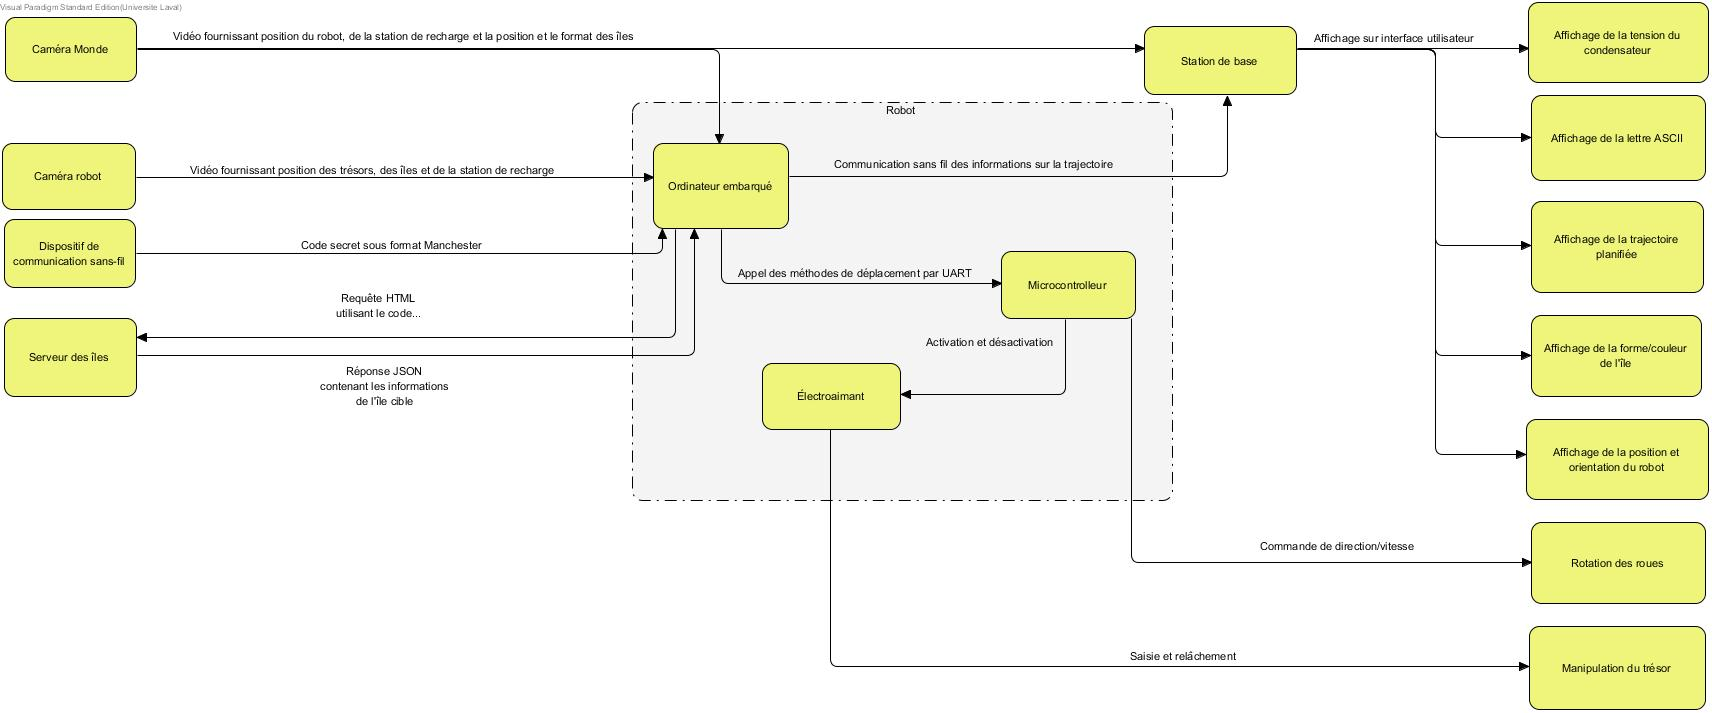
\includegraphics[width=1\textwidth]{fig/contextDiagram.jpg}
   \caption{Diagramme de contexte}
   \label{f:Diagramme_contexte}
\end{figure}

\section{Description des propri�t�s fonctionnelles}

\begin{figure}[htp]
	\centering
	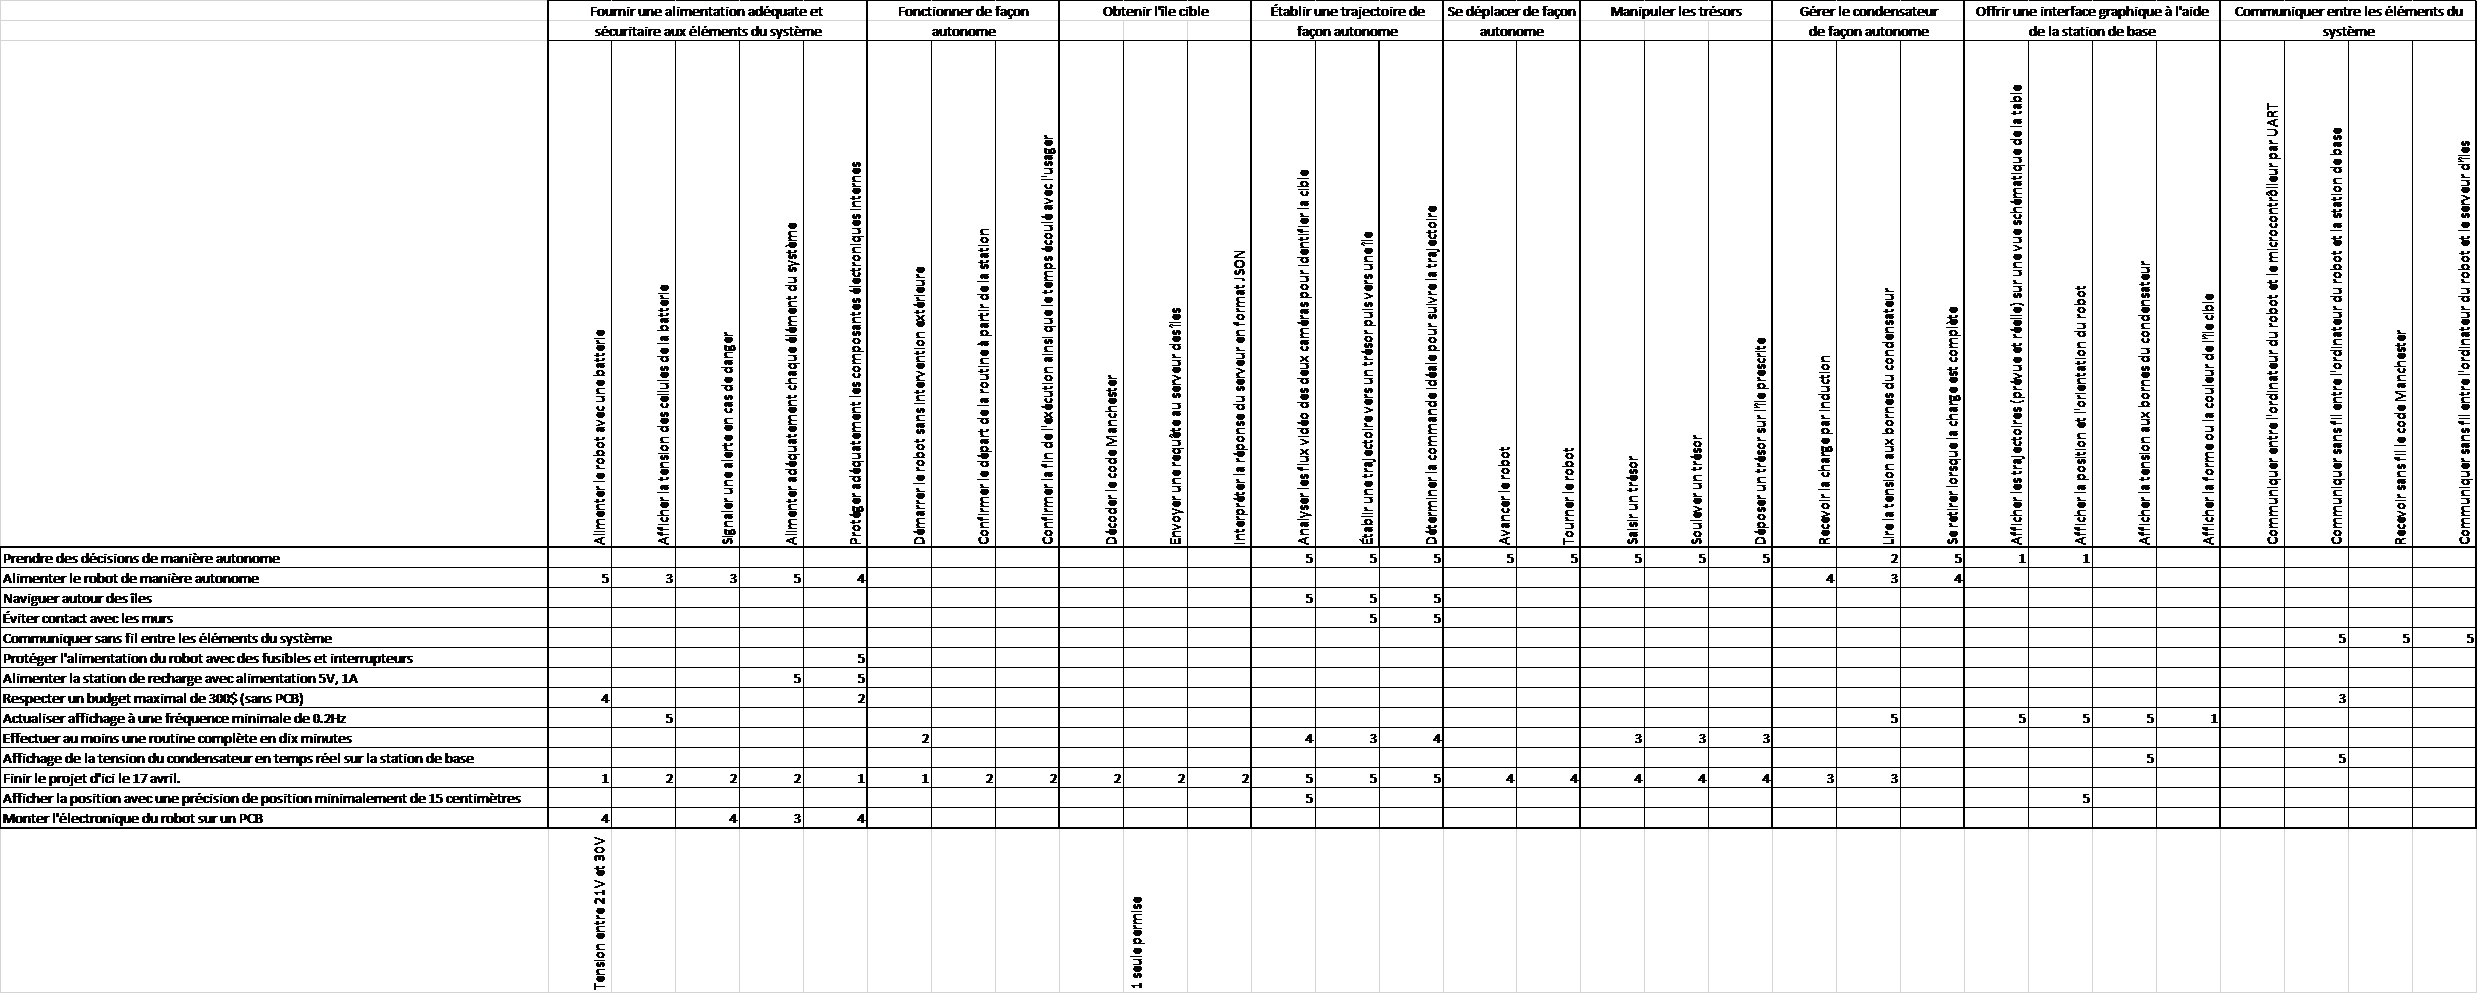
\includegraphics[width=1.3\textwidth, angle =-90]{fig/descriptionPropriete.png}
	\caption{Description des propri�t�s fonctionnelles}
	\label{f:Desc_proprietes}
\end{figure}


\section{Diagrammes de classes}
\label{s:Diagramme_classes}


%\begin{figure}[htp]
%   \centering
%   \includegraphics[width=1\textwidth]{Diagramme_Classes}
%   \caption{Diagrammes de classes}
%   \label{f:Diagrammes_Classes}
%\end{figure}


\section{Diagrammes de s�quences}
\label{s:Diagramme_sequences}


%\begin{figure}[htp]
%   \centering
%   \includegraphics[width=1\textwidth]{Diagrammes_sequences}
%   \caption{Diagrammes de s�quences}
%   \label{f:Diagrammes_sequences}
%\end{figure}

